%% -*- TeX-engine: luatex; ispell-language: "russian" -*-

\documentclass[a4paper,12pt]{article}
\usepackage{subcaption}
\usepackage[left=1.5cm,right=2cm,top=1.5cm,bottom=2cm]{geometry}

\usepackage{parskip}
\setlength{\parindent}{0mm}
\setcounter{secnumdepth}{1}

\usepackage{amsmath}

\usepackage{graphicx}

\usepackage{fontspec}
\setmainfont{PT Serif}
\newfontfamily\cyrillicfont[Script=Cyrillic,Ligatures=TeX]{PT Serif}
\setsansfont{PT Sans}
\setmonofont[Ligatures=NoCommon]{PT Mono}
\defaultfontfeatures{Ligatures=TeX}

\usepackage[bold-style=ISO]{unicode-math}
\setmathfont{XITS Math}

\usepackage{microtype}

\usepackage{hyperref}

\usepackage{polyglossia}
\setmainlanguage{russian}
\setotherlanguage{english}

\usepackage{csquotes}

%% for code snippets
\usepackage{minted}
\newminted[pycon]{pycon}{fontsize=\footnotesize}
\newminted[python3]{python3}{fontsize=\footnotesize}
\newminted[bash]{bash}{fontsize=\footnotesize}
\newmintinline[pythoninline]{python3}{fontsize=\footnotesize}
\newmintinline[bashinline]{bash}{fontsize=\footnotesize}

\pagestyle{empty}


\newcounter{mypar}
\newcommand{\mypar}{\stepcounter{mypar}\paragraph{\arabic{mypar}.}}

\begin{document}
\subsection*{Домашнее задание №6: <<Каракули и нейросети>>}

\begin{tabular}{@{}lr}
  \textbf{Дедлайн 1} (20 баллов): & 9 апреля, 23:59 \\
  \textbf{Дедлайн 2} (10 баллов): & 16 апреля, 23:59
\end{tabular}

Домашнее задание нужно написать на Python и сдать в виде одного файла.
Правило именования файла: \texttt{name\_surname\_6.[py | ipnb]}. Например, если
вас зовут Иван Петров, то имя файла должно быть: \texttt{ivan\_petrov\_6.py} или \texttt{ivan\_petrov\_6.ipnb}.

\makebox[\linewidth]{\hrulefill}

\begin{figure}[h!]
  \centering
  
\includegraphics[width=.7\linewidth]{images/images}
\end{figure}


В этом домашнем задании мы продолжим тему распознавания образов. Для тестирования нашего алгоритма будем использовать датасет MNIST \footnote{\url{http://en.wikipedia.org/wiki/MNIST_database}}. 

MNIST (Mixed National Institute of Standards and Technology database) является основной базой при тестировании систем распознавания образов, а также широко используемой для обучения и тестирования алгоритмов машинного обучения. Она была создана перегруппировкой образов из оригинальной базы NIST, которая являлась достаточно сложной для распознавания. Кроме этого, были выполнены определенные преобразования (образы были нормализованы и сглажены для получения градаций серого цвета). 

\mypar По ссылке \footnote{\url{https://github.com/amplab/datascience-sp14/raw/master/lab7/mldata/mnist-original.mat}} находится датасет для текущего домашнего задания. Данные находятся в формате *.mat, поэтому лучше всего воспользоваться встроенной функцией \pythoninline{scipy.io.loadmat} для чтения данных:

\begin{python3}
import scipy.io
from sklearn.cross_validation import train_test_split

dataset = scipy.io.loadmat('mnist-original.mat')
trainX, testX, trainY, testY = train_test_split(
    dataset['data'].T / 255.0, dataset['label'].squeeze().astype("int0"), test_size = 0.3)
\end{python3}

\mypar Перед работой всегда хорошо бы посмотреть на датасет. Для визуализации датасета можно воспользоваться функцией \pythoninline{visualize_mnist} из файла по ссылке. \footnote{\url{https://gist.github.com/ktisha/95fcee0ed79236c7e6e5}} 

Картинка должна выглядеть подобным образом:

\begin{figure}[h!]
  \centering
  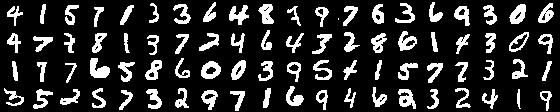
\includegraphics[width=.7\linewidth]{images/mnist}
\end{figure}

\mypar Реализуйте обучение нейронной сети с помощью метода обратного распространения ошибки (Back Propagation). 

В качестве функции активации в данном задании допустимо воспользоваться сигмоидой, функцию потерь нужно взять из лекции.

Структура класса приведена ниже:
\begin{python3}	
class NeuralNetwork:
    def __init__(self, layers):
        self.num_layers = len(layers)
        self.layers = layers
        ...

    def train(self, X, y, max_iter=10000, learning_rate=1): 
        ...
        for j in range(max_iter):
          self.forward(X)
          self.backward(X, y)
          ...
        
    def forward(self, X): 
        ...
        
    def backward(self, X, y):
        ...
    	
    def predict(self, X):
        ...

\end{python3}
Параметр конструктора \pythoninline{layers} задаёт количество нейронов в каждом слое в виде списка. 

На \pythoninline{forward} шаге объект проходит через нейросеть и вычисляются выходные значения нейронов скрытых слоёв и выходного слоя. На \pythoninline{backward} шаге вычисляются производные, необходимые для обновления массива весов. 

При реализации метода \pythoninline{train} может быть полезно обратиться к своей реализации метода стохастического градиента из предыдущего домашнего задания. 

\mypar Дополните реализацию методом \pythoninline{predict}, который прогоняет все объекты из переданной матрицы \pythoninline{X} через обученную нейросеть. Метод должен возвращать вектор, состоящий из индексов нейронов, на котором значение для соответствующего объекта на выходном слое максимально.

\mypar Пример использования полученной сети:
\begin{python3}
nn = NeuralNetwork([train_X.shape[1], 100, 10])
nn.train(trainX, trainY)
nn.predict(testY)
\end{python3}
Обратите внимание, что на первом слое нам нужно число нейронов, равное количеству признаков (в данном случае, количеству пикселей), а на выходном слое количество нейронов, равное количеству классов объектов (в нашем случае это цифры 0-9).

\mypar Оценивать качество классификации в этот раз мы будем с помощью простым подсчетом отношения правильно классифицированных объектов к общему количеству объектов в выборке.

\mypar Ответьте на вопрос: как меняется качество классификации при изменении количества слоев сети и количества нейронов на каждом слое?
 
\end{document}
